%  LaTeX support: latex@mdpi.com 
%  For support, please attach all files needed for compiling as well as the log file, and specify your operating system, LaTeX version, and LaTeX editor.

%=================================================================
\documentclass[journal,article,submit,pdftex,moreauthors]{Definitions/mdpi} 

%--------------------
% Class Options:
%--------------------
%----------
% journal
%----------
% Choose between the following MDPI journals:
% acoustics, actuators, addictions, admsci, adolescents, aerobiology, aerospace, agriculture, agriengineering, agrochemicals, agronomy, ai, air, algorithms, allergies, alloys, analytica, analytics, anatomia, animals, antibiotics, antibodies, antioxidants, applbiosci, appliedchem, appliedmath, applmech, applmicrobiol, applnano, applsci, aquacj, architecture, arm, arthropoda, arts, asc, asi, astronomy, atmosphere, atoms, audiolres, automation, axioms, bacteria, batteries, bdcc, behavsci, beverages, biochem, bioengineering, biologics, biology, biomass, biomechanics, biomed, biomedicines, biomedinformatics, biomimetics, biomolecules, biophysica, biosensors, biotech, birds, bloods, blsf, brainsci, breath, buildings, businesses, cancers, carbon, cardiogenetics, catalysts, cells, ceramics, challenges, chemengineering, chemistry, chemosensors, chemproc, children, chips, cimb, civileng, cleantechnol, climate, clinpract, clockssleep, cmd, coasts, coatings, colloids, colorants, commodities, compounds, computation, computers, condensedmatter, conservation, constrmater, cosmetics, covid, crops, cryptography, crystals, csmf, ctn, curroncol, cyber, dairy, data, ddc, dentistry, dermato, dermatopathology, designs, devices, diabetology, diagnostics, dietetics, digital, disabilities, diseases, diversity, dna, drones, dynamics, earth, ebj, ecologies, econometrics, economies, education, ejihpe, electricity, electrochem, electronicmat, electronics, encyclopedia, endocrines, energies, eng, engproc, entomology, entropy, environments, environsciproc, epidemiologia, epigenomes, est, fermentation, fibers, fintech, fire, fishes, fluids, foods, forecasting, forensicsci, forests, foundations, fractalfract, fuels, future, futureinternet, futurepharmacol, futurephys, futuretransp, galaxies, games, gases, gastroent, gastrointestdisord, gels, genealogy, genes, geographies, geohazards, geomatics, geosciences, geotechnics, geriatrics, grasses, gucdd, hazardousmatters, healthcare, hearts, hemato, hematolrep, heritage, higheredu, highthroughput, histories, horticulturae, hospitals, humanities, humans, hydrobiology, hydrogen, hydrology, hygiene, idr, ijerph, ijfs, ijgi, ijms, ijns, ijpb, ijtm, ijtpp, ime, immuno, informatics, information, infrastructures, inorganics, insects, instruments, inventions, iot, j, jal, jcdd, jcm, jcp, jcs, jcto, jdb, jeta, jfb, jfmk, jimaging, jintelligence, jlpea, jmmp, jmp, jmse, jne, jnt, jof, joitmc, jor, journalmedia, jox, jpm, jrfm, jsan, jtaer, jvd, jzbg, kidneydial, kinasesphosphatases, knowledge, land, languages, laws, life, liquids, literature, livers, logics, logistics, lubricants, lymphatics, machines, macromol, magnetism, magnetochemistry, make, marinedrugs, materials, materproc, mathematics, mca, measurements, medicina, medicines, medsci, membranes, merits, metabolites, metals, meteorology, methane, metrology, micro, microarrays, microbiolres, micromachines, microorganisms, microplastics, minerals, mining, modelling, molbank, molecules, mps, msf, mti, muscles, nanoenergyadv, nanomanufacturing,\gdef\@continuouspages{yes}} nanomaterials, ncrna, ndt, network, neuroglia, neurolint, neurosci, nitrogen, notspecified, %%nri, nursrep, nutraceuticals, nutrients, obesities, oceans, ohbm, onco, %oncopathology, optics, oral, organics, organoids, osteology, oxygen, parasites, parasitologia, particles, pathogens, pathophysiology, pediatrrep, pharmaceuticals, pharmaceutics, pharmacoepidemiology,\gdef\@ISSN{2813-0618}\gdef\@continuous pharmacy, philosophies, photochem, photonics, phycology, physchem, physics, physiologia, plants, plasma, platforms, pollutants, polymers, polysaccharides, poultry, powders, preprints, proceedings, processes, prosarticle, proteomes, psf, psych, psychiatryint, psychoactives, publications, quantumrep, quaternary, qubs, radiation, reactions, receptors, recycling, regeneration, religions, remotesensing, reports, reprodmed, resources, rheumato, risks, robotics, ruminants, safety, sci, scipharm, sclerosis, seeds, sensors, separations, sexes, signals, sinusitis, skins, smartcities, sna, societies, socsci, software, soilsystems, solar, solids, spectroscj, sports, standards, stats, std, stresses, surfaces, surgeries, suschem, sustainability, symmetry, synbio, systems, targets, taxonomy, technologies, telecom, test, textiles, thalassrep, thermo, tomography, tourismhosp, toxics, toxins, transplantology, transportation, traumacare, traumas, tropicalmed, universe, urbansci, uro, vaccines, vehicles, venereology, vetsci, vibration, virtualworlds, viruses, vision, waste, water, wem, wevj, wind, women, world, youth, zoonoticdis 
% For posting an early version of this manuscript as a preprint, you may use "preprints" as the journal. Changing "submit" to "accept" before posting will remove line numbers.

%---------
% article
%---------
% The default type of manuscript is "article", but can be replaced by: 
% abstract, addendum, article, book, bookreview, briefreport, casereport, comment, commentary, communication, conferenceproceedings, correction, conferencereport, entry, expressionofconcern, extendedabstract, datadescriptor, editorial, essay, erratum, hypoarticle, interestingimage, obituary, opinion, projectreport, reply, retraction, review, perspective, protocol, shortnote, studyprotocol, systematicreview, supfile, technicalnote, viewpoint, guidelines, registeredreport, tutorial
% supfile = supplementary materials

%----------
% submit
%----------
% The class option "submit" will be changed to "accept" by the Editorial Office when the paper is accepted. This will only make changes to the frontpage (e.g., the logo of the journal will get visible), the headings, and the copyright information. Also, line numbering will be removed. Journal info and pagination for accepted papers will also be assigned by the Editorial Office.

%------------------
% moreauthors
%------------------
% If there is only one author the class option oneauthor should be used. Otherwise use the class option moreauthors.

%---------
% pdftex
%---------
% The option pdftex is for use with pdfLaTeX. Remove "pdftex" for (1) compiling with LaTeX & dvi2pdf (if eps figures are used) or for (2) compiling with XeLaTeX.

%=================================================================
% MDPI internal commands - do not modify
\firstpage{1} 
\makeatletter 
\setcounter{page}{\@firstpage} 
\makeatother
\pubvolume{1}
\issuenum{1}
\articlenumber{0}
\pubyear{2023}
\copyrightyear{2023}
%\externaleditor{Academic Editor: Firstname Lastname}
\datereceived{ } 
\daterevised{ } % Comment out if no revised date
\dateaccepted{ } 
\datepublished{ } 
%\datecorrected{} % For corrected papers: "Corrected: XXX" date in the original paper.
%\dateretracted{} % For corrected papers: "Retracted: XXX" date in the original paper.
\hreflink{https://doi.org/} % If needed use \linebreak
%\doinum{}
%\pdfoutput=1 % Uncommented for upload to arXiv.org

%=================================================================
% Add packages and commands here. The following packages are loaded in our class file: fontenc, inputenc, calc, indentfirst, fancyhdr, graphicx, epstopdf, lastpage, ifthen, float, amsmath, amssymb, lineno, setspace, enumitem, mathpazo, booktabs, titlesec, etoolbox, tabto, xcolor, colortbl, soul, multirow, microtype, tikz, totcount, changepage, attrib, upgreek, array, tabularx, pbox, ragged2e, tocloft, marginnote, marginfix, enotez, amsthm, natbib, hyperref, cleveref, scrextend, url, geometry, newfloat, caption, draftwatermark, seqsplit
% cleveref: load \crefname definitions after \begin{document}

%=================================================================
% Please use the following mathematics environments: Theorem, Lemma, Corollary, Proposition, Characterization, Property, Problem, Example, ExamplesandDefinitions, Hypoarticle, Remark, Definition, Notation, Assumption
%% For proofs, please use the proof environment (the amsthm package is loaded by the MDPI class).

%=================================================================
% Full title of the paper (Capitalized)
\Title{Model Based Systems Engineering with a Docs-as-Code Approach for the SeaLion CubeSat Project}

% MDPI internal command: Title for citation in the left column
\TitleCitation{Title}

% Author Orchid ID: enter ID or remove command
\newcommand{\orcidauthorA}{0000-0000-0000-000X} % Add \orcidA{} behind the author's name
%\newcommand{\orcidauthorB}{0000-0000-0000-000X} % Add \orcidB{} behind the author's name

% Authors, for the paper (add full first names)
\Author{Kevin Chiu $^{1,\dagger,\ddagger}$\orcidA{}, Sean Marquez $^{2,\ddagger}$ and Sharanabasaweshwara Asundi, PhD. $^{2,}$*}

%\longauthorlist{yes}

% MDPI internal command: Authors, for metadata in PDF
\AuthorNames{Kevin Chiu, Sean Marquez, and Sharanabasaweshwara Asundi}

% MDPI internal command: Authors, for citation in the left column
\AuthorCitation{Chiu K.; Marquez, S.; Asundi, A.}
% If this is a Chicago style journal: Lastname, Firstname, Firstname Lastname, and Firstname Lastname.

% Affiliations / Addresses (Add [1] after \address if there is only one affiliation.)
\address{%
$^{1}$ \quad Old Dominion University; kchiu002@odu.edu\\
$^{2}$ \quad Old Dominion University; sasundi@odu.edu}

% Contact information of the corresponding author
\corres{Correspondence: kchiu002@odu.edu}

% Current address and/or shared authorship
\firstnote{Old Dominion University: Norfolk, VA, 23529, USA} 
\secondnote{These authors contributed equally to this work.}

% Contact information of the corresponding author
%\corres{Correspondence: e-mail@e-mail.com; Tel.: (optional; include country code; if there are multiple corresponding authors, add author initials) +xx-xxxx-xxx-xxxx (F.L.)}

% Current address and/or shared authorship
%\firstnote{Current address: Affiliation 3.} 
%\secondnote{These authors contributed equally to this work.}
% The commands \thirdnote{} till \eighthnote{} are available for further notes

%\simplesumm{} % Simple summary

%\conference{} % An extended version of a conference paper

% Abstract (Do not insert blank lines, i.e. \\) 
\abstract{The SeaLion mission architecture team sought to create a model based systems engineering approach to assist improving CubeSat success rates as well as for the SeaLion CubeSat project to guide an implementation for the flight software.  Especially as university CubeSat teams grow in number but are characterized with having untrained students as their core personnel.  This was done using a document-as-code, or docs-as-code, approach.  With this the team created tools for the systems architecture with the Mach 30 Modeling Language to create a architecture that is easy to learn and use even for newly admitted team members with little to no training. These tools generate documents via its own code for easy presentaton on a local file system without any proprietary software while keeping model content format-agnostic.}

% Keywords
\keyword{systems engineering; CubeSat; MBSE} 

% The fields PACS, MSC, and JEL may be left empty or commented out if not applicable
%\PACS{J0101}
%\MSC{}
%\JEL{}

%%%%%%%%%%%%%%%%%%%%%%%%%%%%%%%%%%%%%%%%%%
% Only for the journal Diversity
%\LSID{\url{http://}}

%%%%%%%%%%%%%%%%%%%%%%%%%%%%%%%%%%%%%%%%%%
% Only for the journal Applied Sciences
%\featuredapplication{Authors are encouraged to provide a concise description of the specific application or a potential application of the work. This section is not mandatory.}
%%%%%%%%%%%%%%%%%%%%%%%%%%%%%%%%%%%%%%%%%%

%%%%%%%%%%%%%%%%%%%%%%%%%%%%%%%%%%%%%%%%%%
% Only for the journal Data
%\dataset{DOI number or link to the deposited data set if the data set is published separately. If the data set shall be published as a supplement to this paper, this field will be filled by the journal editors. In this case, please submit the data set as a supplement.}
%\datasetlicense{License under which the data set is made available (CC0, CC-BY, CC-BY-SA, CC-BY-NC, etc.)}

%%%%%%%%%%%%%%%%%%%%%%%%%%%%%%%%%%%%%%%%%%
% Only for the journal Toxins
%\keycontribution{The breakthroughs or highlights of the manuscript. Authors can write one or two sentences to describe the most important part of the paper.}

%%%%%%%%%%%%%%%%%%%%%%%%%%%%%%%%%%%%%%%%%%
% Only for the journal Encyclopedia
%\encyclopediadef{For entry manuscripts only: please provide a brief overview of the entry title instead of an abstract.}

%%%%%%%%%%%%%%%%%%%%%%%%%%%%%%%%%%%%%%%%%%
% Only for the journal Advances in Respiratory Medicine
%\addhighlights{yes}
%\renewcommand{\addhighlights}{%

%\noindent This is an obligatory section in “Advances in Respiratory Medicine”, whose goal is to increase the discoverability and readability of the article via search engines and other scholars. Highlights should not be a copy of the abstract, but a simple text allowing the reader to quickly and simplified find out what the article is about and what can be cited from it. Each of these parts should be devoted up to 2~bullet points.\vspace{3pt}\\
%\textbf{What are the main findings?}
% \begin{itemize}[labelsep=2.5mm,topsep=-3pt]
% \item First bullet.
% \item Second bullet.
% \end{itemize}\vspace{3pt}
%\textbf{What is the implication of the main finding?}
% \begin{itemize}[labelsep=2.5mm,topsep=-3pt]
% \item First bullet.
% \item Second bullet.
% \end{itemize}
%}

%%%%%%%%%%%%%%%%%%%%%%%%%%%%%%%%%%%%%%%%%%
\begin{document}

%%%%%%%%%%%%%%%%%%%%%%%%%%%%%%%%%%%%%%%%%%
% The order of the section titles is different for some journals. Please refer to the "Instructions for Authors” on the journal homepage.

\section{Introduction}

Presented here is the systems engineering approach of the SeaLion CubeSat mission architecture.  This includes the modeling language, tools, and technical approach used to facilitate the configuration management, design, specification, and implementation of the SeaLion mission architecture for the flight software using a model-based approach.  Through, model-based systems engineering (MBSE), the SeaLion mission architecture team was able to create models, as opposed to documents, that serve as the authoritative source of truth for the conduction of system engineer activities \cite{architecting_spacecraft}.  These models were used to conduct activities such as design, specification, analysis, verification, and validation of the system.  This was done by applying the NASA handbook on systems engineering \cite{nasa_handbook} to CubeSat mission design in efforts to facilitate a top-down design methodology from mission concept to specification of subsystem components, including flight software architecture \cite{asundi13_cubes}.  The approach presented herein had additional intents to make it as simple and easy to use as possible.  This was done by a filesystem-based modelling language that adheres to expected patterns in agile software engineering (i.e., elements for stakeholder needs, user stories, data structures, etc.) using a lightweight YAML-based syntax.  This article also serves as an expansion of the conference proceedings (copyright held by Kevin Chiu and Sean Marquez) presented at American Institute of Aeronautics and Astronautics (AIAA) SciTech Forum 2023 \cite{scitech_proceeding}.

\subsection{CubeSat}
The CubeSat, originating from California Polytechnic State University in 1999, is a standardized form of nanosatellites.  Nanosatellites are satellites typically defined with a mass of less than 10 kg.  CubeSats, also known as Cube Satellites, are defined by the standardized and modular architecture of a 1-Unit (1U) cube with dimensions of 10 cm X 10 cm X 10 cm with a mass of up to 2 kg \cite{cds_rev14}.  They can be scaled to 2-Units (2U), 3-Units (3U), or higher depending on units added as shown in figure \ref{fig:cubesat_family} with sizes designated by the CubeSat specification \cite{cds_rev14}.  This is done by the addition of standardized cube units to upscale the CubeSat.  The ability to scale by modularity gives a highly standardized structure for ease of expansion to provide versatility in functionality.  Due to their small size, mass, and lack of dedicated launch vehicles, CubeSats are typically launched as secondary payloads in conjunction with other larger satellites, informally known as “piggy-backing”.  This greatly decreases the cost of launching a CubeSat which increases the accessibility of inserting objects into space.  As such, low budget groups such as universities have gravitated towards CubeSats with increasing numbers \cite{swartwout_data}.  However, this presents challenges since many of the developers in universities are completely new to spacecraft development or systems engineering in general.

\begin{figure}[H]
    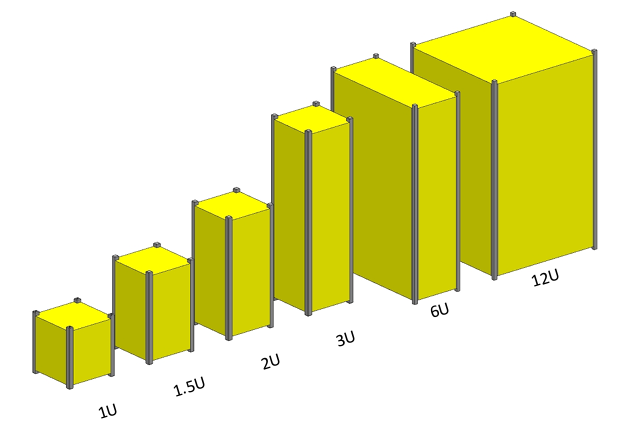
\includegraphics[width=10.5 cm]{assets/cubesat_family.png}
    \caption{CubeSat family by size \cite{cds_rev14}}
	\label{fig:cubesat_family}
    \end{figure}   
\unskip

\subsection{SeaLion Mission}
The SeaLion CubeSat mission is a joint project between Old Dominion University (ODU), the United States Coast Guard Academy (USCGA), and the Air Force Institute of Technology (AFIT).  The end goal is to produce a 3U CubeSat consisting of 3 payloads for on-orbit validation.  ODU provided one payload while the USCGA and AFIT provided the other two payloads.  SeaLion was initially planned to launch as a secondary payload on a Northrop Grumman Antares Rocket from Wallops Flight Facility (WFF) during March of 2023 \cite{sealion_cdr}.  The prototype CubeSat model is shown in figure \ref{fig:cubesat_blowup}.  The intended mission profile was to have an on-orbit time for mere days due to its planned very low earth orbit (VLEO) altitude.  Thus, SeaLion was to complete validation of its payloads before either power is lost in its non-rechargeable batteries or the satellite reenters and burns up in Earth's atmosphere.  The predicted on-orbit time was 10 days.  However, mass considerations on the planned Antares rocket caused SeaLion to be moved to a Q4 2023 launch on a Firefly rocket from Vandenberg Space Force Base into a sun synchronous orbit, of 500 miles altitude.  The content presented in this article is based on the prior mission profile from the launch at WFF into VLEO.

\begin{figure}[H]
    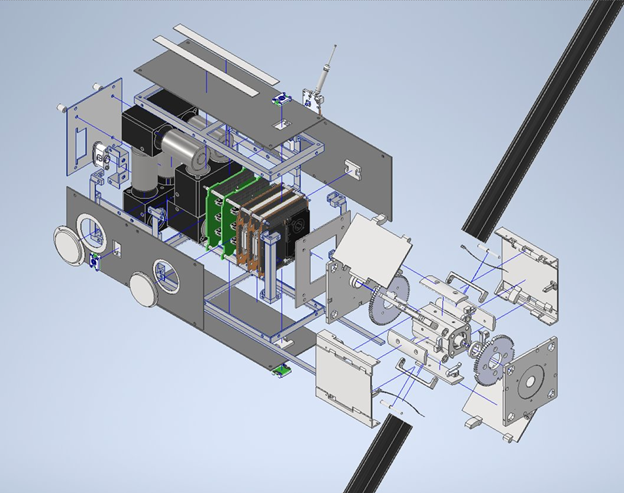
\includegraphics[width=10.5 cm]{assets/cubesat_blownup.png}
    \caption{Blownup SeaLion CubeSat Prototype}
	\label{fig:cubesat_blowup}
    \end{figure}
	\noindent   
\unskip

The first payload, provided by the USCGA and AFIT, is the Impedance Probe (IP).  The IP is derived from U.S. Naval Research Laboratory's (NRL's) 'Space PlasmADiagnostic suitE' (SPADE) aboard NASA's International Space Station (ISS) where plasma density and temperature are computed with alternating current (AC) impedance measurements using an innovative, first of its kind surface mounted dipole radio frequency antenna \cite{sealion_cdr}.  The IP part is shown in figure \ref{fig:IP}.

\begin{figure}[H]
    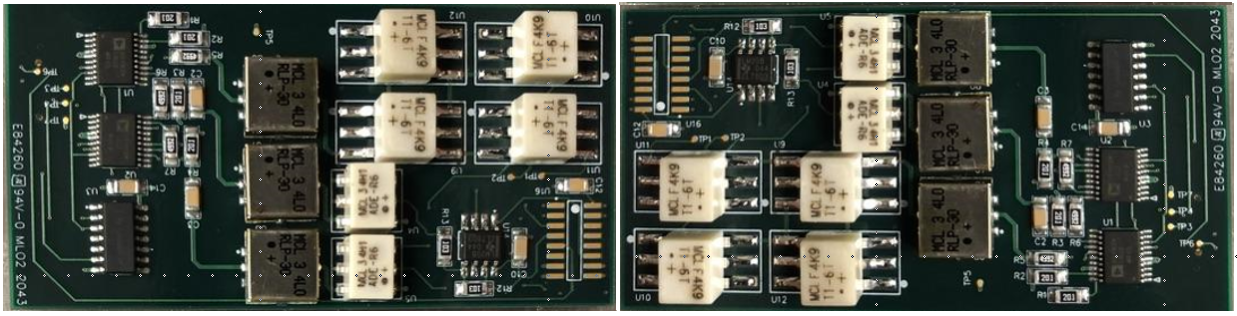
\includegraphics[width=13.75 cm]{assets/impedence.png}
    \caption{Impedence Probe}
	\label{fig:IP}
    \end{figure}
	\noindent   
\unskip

The second payload, provided by the USCGA and AFIT, is the multispectral (Me-S) 'Pixel Sensor' with a 450 nm - 1000 nm spectral range \cite{sealion_cdr}.  Its purpose is to provide SeaLion's in-situ spectral data as a baseline.  This baseline will be used for future missions that may require this spectral data.  The Me-S part is shown in figure \ref{fig:Me-S}. 

\begin{figure}[H]
    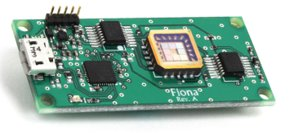
\includegraphics{assets/spectral.png}
    \caption{Me-S 'Pixel Sensor'}
	\label{fig:Me-S}
    \end{figure}
	\noindent   
\unskip

The third payload, provided by ODU, is the deployable composite structure (DeCS).  This payload is a proof-of-concept deployable mechanism and composite boom that is meant to be a platform host of a number of applications \cite{sealion_cdr}.  For example, these applications include solar panels, solar sails, drag sails, sensory sails, and magnetometer booms.  Deployment on SeaLion is meant to validate the deployable mechanism for a composite boom in the space environment and to validate boom dynamics during and after deployment in orbit.  The DeCS upon deployment is shown in figure \ref{fig:DeCS}.

\begin{figure}[H]
    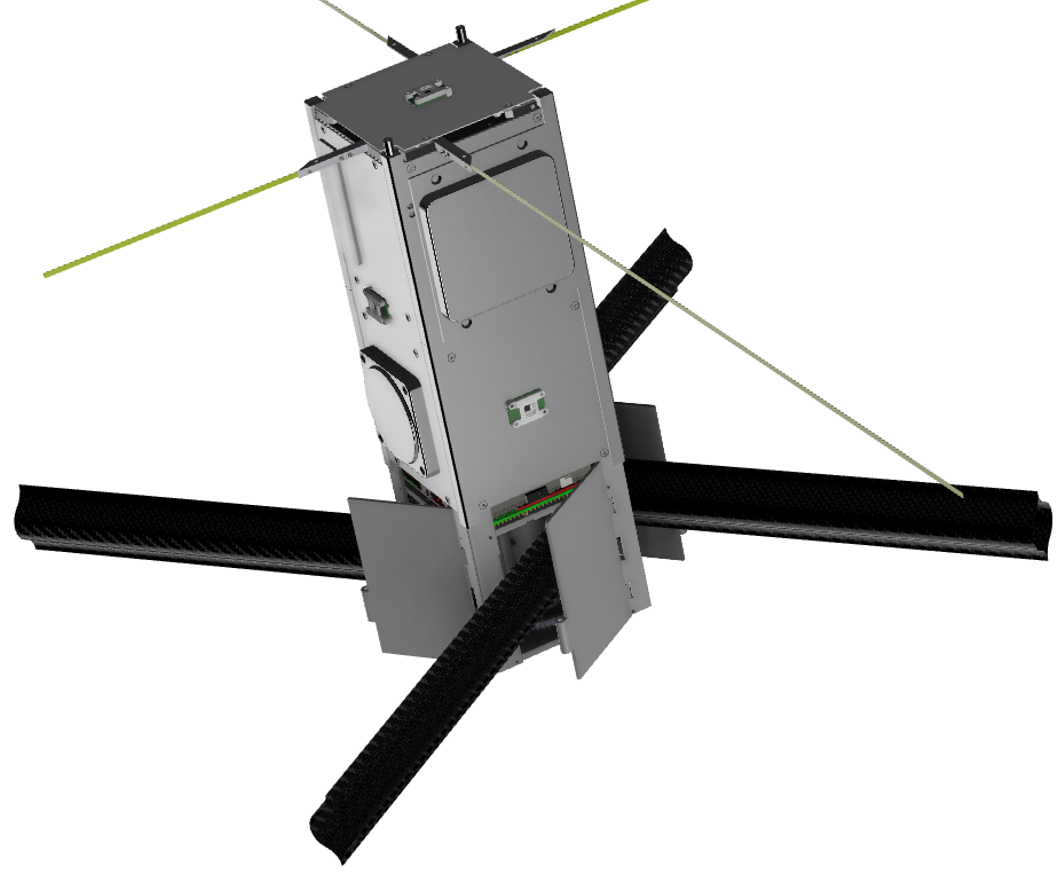
\includegraphics[width=13.75 cm]{assets/decs.png}
    \caption{DeCS as the black popout booms}
	\label{fig:DeCS}
    \end{figure}
	\noindent   
\unskip

The mission scope with three payloads requires special care and attention to ensure success of the mission.  However, many of the SeaLion project team members are new to spacecraft development and systems engineering.  In response, experienced team members took action to provide a mission architecture for the SeaLion team to better organize and direct the efforts of the team, to guide an implementation for the flight software, and to facilitate interface and assembly documentation.

%%%%%%%%%%%%%%%%%%%%%%%%%%%%%%%%%%%%%%%%%%
\section{Motivation}
\subsection{CubeSat Populations}

CubeSats were initially conceived as educational tools for space systems engineering \cite{heidt_new}.  Now, their roles have been expanded to not only just educational tools but for observation, technology demonstrations, and research that were previous monopolized by much larger satellites due to the low cost of production and launch of these CubeSats.  As such, there has been increasing popularity for CubeSats as seen by the number of launches in figure \ref{fig:launch_data} since the year 2000 \cite{swartwout_data} apart from the notable exceptions in the years 2020 and 2021; the author speculates that this downturn is due to the COVID-19 pandemic.  The CubeSat design specification \cite{cds_rev14} as well as the availability of commercial off-the-shelf (COTS) parts and kits have greatly influenced the rise of popularity.  For example, a basic CubeSat kit from a space systems company such as Pumpkin can be purchased with a baseline price of as little as 6250 US dollars \cite{pumpkin_cubesat}.  The SeaLion CubeSat also utilizes many COTS parts as well.  Thus, CubeSats have become highly accessible to low-budget groups such as small companies and university groups.  CubeSats have caused the “democratization” of space by allowing many groups to fly satellites \cite{cubesat_handbook}.  

\begin{figure}[H]
    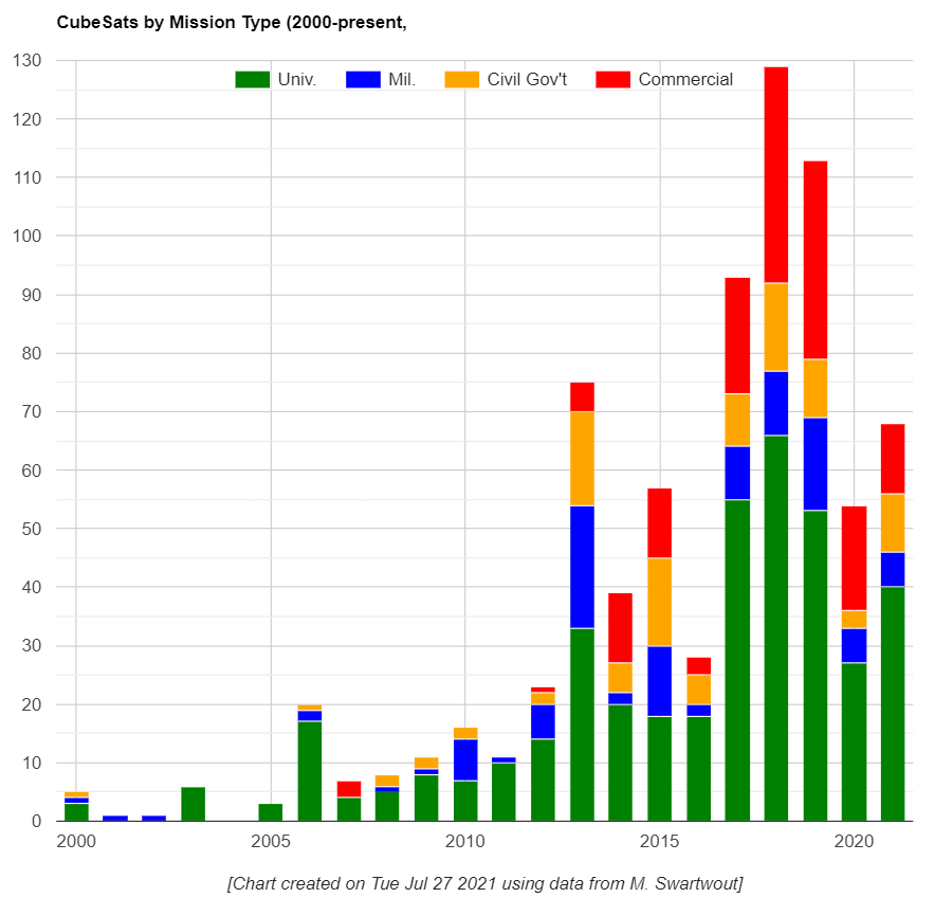
\includegraphics[width=13.75 cm]{assets/launch_data.png}
    \caption{Nanosatellite launch data provided by M. Swartwout as of July 21, 2021 \cite{swartwout_data}}
	\label{fig:launch_data}
    \end{figure}
	\noindent   
\unskip

University groups especially are a large contributor in the overall number of launches of CubeSats yearly.  As of July 27, 2021, alone, there have been 68 CubeSat launches with 40 of them being from university groups (about 58 percent of launches) in the year of 2021; university groups have consistently maintained plurality on total launches \cite{swartwout_data}.  This showcases directly how many university-based CubeSat projects occurred or potentially may occur if trends continue onwards into the future.  However, this presents its own challenges.

\subsection{Ensuring CubeSat Success}
The motivation of this article is to improve the success rate of CubeSat missions from university groups by providing readily available and usable tools for university teams.  To further reinforce the need to improve the success rate, the following data is presented in figure \ref{fig:mission_status} which showcases the total successes and failures of CubeSats from universities for the given time periods \cite{reliving_24}.  The data provided is categorized by six different mission success statuses of unknown, launch fail, dead on arrival (DOA), early loss, partial mission, and full mission.

\begin{figure}[H]
    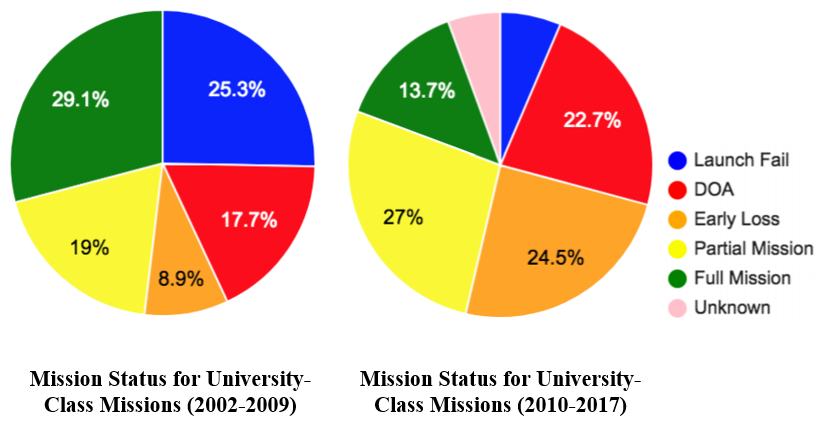
\includegraphics[width=10.5 cm]{assets/mission_status.png}
    \caption{Mission status of CubeSat university-class missions provided by Swartwout \cite{reliving_24}}
	\label{fig:mission_status}
    \end{figure}
	\noindent   
\unskip

As seen in the preceding figure \ref{fig:mission_status}, university CubeSat mission failure rates have increased while partial and full mission success rates have decreased in conjunction with the increasing number of missions as seen in figure \ref{fig:launch_data}.  However, Swartwout notes that the highest number of failures originate from “regular independent” groups with a failure rate of 65 percent at the time of data gathering in 2017 \cite{reliving_24}.  These “regular independent” groups have fewer than four missions performed nor are designated as a national center for spacecraft development by its government. 

The issue present is that many of the growing number of university groups producing CubeSats lack the resources, training, experience, or methodology to reliably give assurance to their missions.  The majority of the work is often done by untrained students that are unfamiliar with the aspects of CubeSat development (e.g., system engineering, design methods, and testing).  The SeaLion team also faced these issues as well.

To address some of these issues, SeaLion team members sought to simplify the development process by providing readily available and learnable system engineering approaches and tools.  These provided approaches and tools include factors such as planning, documentation, project management, and simplifying the process.  This is important since special attention should be given to systems engineering and information exchange for multidisciplinary teams \cite{aalto}.  To showcase these factor's importance, a survey of forty CubeSat groups on how to set up CubeSat projects, conducted by the University of Bristol, emphasized the following relevant lessons learned \cite{howtosetup}:

\begin{itemize}
	\item	Planning: Make efforts to “spend a lot of time in the planning stage”.;
	\item	Documentation / Project Management: Groups should have “good documentation of requirements, work done and work to do”.;
	\item	Simplicity: Simplify anything you possibly can to increase confidence in success.
\end{itemize}

The developed mission architecture and associated tools will emphasize the aforementioned points to further the SeaLion CubeSat's development.

%%%%%%%%%%%%%%%%%%%%%%%%%%%%%%%%%%%%%%%%%%
\section{Goals}

The goal of the SeaLion CubeSat mission architecture was to capture the data structures and expected behaviors for the development of the flight software.  The data structures and expected behaviors were captured in such a way that can unambiguously understood well enough to be implemented, as well as provide full traceability and rationale for architectural elements with minimal configuration management overhead \cite{sealion_mission_architecture}.  Thus, the SeaLion CubeSat mission architecture had to achieve the following:

\begin{itemize}
	\item	Ensure templates only contain formatting data (this includes not storing boilerplate text in templates);
	\item	Ensure models are the authoritative source of truth for all artifact content (e.g., artifact structure, meta-data, boilerplate, commentary, discussion, diagrams, tables, etc.);
	\item 	Models should persist on the local filesystem.;
	\item 	Documents should be in plaintext as to be compatible with modern distributed version control system (e.g., Git) and for ease of use.;
	\item 	Documents should be able to persist alongside code and communicate to one another.;
	\item 	Documents should be model-based as to have a separation of concerns between content and formatting as well as be both human and machine-readable for querying and generating views.;
\end{itemize}

A MBSE approach was adopted by the Sealion CubeSat mission architecture team since it provided benefits such as reducing the ambiguity that usually comes with using informal language to specify systems or its various aspects.  It also minimized the duplication of content that tends to accumulate in a document-based system engineering approach.

Proper adoption of a MBSE approach also includes the selection of the modeling language and modeling tool.  Considerations when selecting the modeling language and tool was overhead incurred from training the team, the technical overhead of setting up modelling tools, and future adaptability.  Refer to table \ref{tab:language} for modelling language down selection overview.  In addition, the Sealion CubeSat mission architecture team eventually decided to adopt a docs-as-code approach to further enhance the MBSE approach to achieve the listed goals shown above.

\subsection{Model-Based Systems Engineering}
As noted prior that attention should be given for planning, documentation, project management, and simplifying the process.  Special emphasize should be given to systems engineering and information exchange \cite{aalto}.

Traditional approaches use documents as their authoritative source of truth for conducting system engineering activities \cite{architecting_spacecraft}.  Information in a traditional systems engineering approach today is mostly captured informally.  For example, it incurs disadvantages such as information not being authored based on a methodology, adhocly and infrequently integrated, not properly configuration managed, not properly changed managed, and not effectively shared with stakeholders \cite{caesar_model_based_approach}.  These documents often do not have a living relationship with other documents or to other corresponding elements; thus, changes to one document require manual changes to other documents \cite{ibm_mbse}.  Document-based approaches can exacerbate problems since it lacks point-to-point communication channels as well as lacking methods to enforce consistency \cite{call_herber_2022}.  

In contrast, a MBSE approach captures information in a highly structured modeling language, authored based on a methodology, configuration managed in a common tool, highly integrated, traceable to its provenance, and sharing with stakeholders.  Models provide the following key advantages over document-based approaches \cite{ibm_mbse}: 

\begin{itemize}
	\item	Information is readily communicated and shared within the project.
	\item	Changes are easily accommodated.
	\item	Traceability is automated.
\end{itemize}

To showcase the benefits, an architecting process of 4,858 information element transfers was performed.  It noted that all of these transfers were done manually with non-MBSE approaches; however, 13\% of these transfers were automated with MBSE with the potential of up to 81\% should it be used for trade study and peer review tasks \cite{younse_cameron_bradley_2021}.  The SeaLion mission architecture team seeks to take advantage of these efficiency gains that MBSE can achieve.  Space projects have been taking advantage of MBSE such as the ExoMars mission, Euclid, Galileo, and nanosatellite programs \cite{mazzini}, \cite{esa}, \cite{nottage_corns_2012}.  CubeSat projects have also been using MBSE and have shown to “hold promise of reducing the burden of system engineering tasks” \cite{kaslow} and can “promote uniformity and consistency across future CubeSat models” \cite{kaslow}.  These attributes are important to reduce workload amongst team members and to facilitate new team members as they join future projects.  Facilitation of new members is especially useful for universities since students are not available long term due to events such as graduation.

\subsection{Documents-As-Code Approach}
Documents-as-code (Docs-as-code) refers to a philosophy that team members should be writing documentation with the same tools as code \cite{docs_as_code}.  This allows for documentation to be updated seamlessly without additional work with document tools (doctools).  The code tools would include version control (e.g., Git), issues trackers, code tools (e.g., Visual Studio Code), etc.  To do so would mean that writers would follow the same workflows as the development team and they would be integrated into the product team.  A stated result would be to enable "a culture where writers and developers both feel ownership of documentation, and work together to make it as good as possible” \cite{docs_as_code}.  The SeaLion team taking advantage of the aforementioned philosophy would realize the benefits of utilizing the same principles and practices used to manage software, using modern version control tools (e.g., Git), for the configuration management of mission and flight software architecture documentation, and captured in a model-based approach \cite{docs_as_code}.  In addition, these models can be stored and used persistently on a local file system without the use of cloud based services.  Proprietary services are not required to generate documentation, modify documentation, or modify models.  Similar approaches have been seen in Structurizr \cite{structurizr} and F Prime Prime (FPP) \cite{f_prime_prime}.  FPP is based on F Prime which is an open-source software framework developed by NASA's Jet Propulsion Laboratory \cite{f_prime}; it is a model-driven approach for producing flight software code that can be compiled directly onto flight hardware.  While docs-as-code has precedent, the methodologies noted are not easily accesible to those without a sufficient background in programming.


%%%%%%%%%%%%%%%%%%%%%%%%%%%%%%%%%%%%%%%%%%
\section{Modelling Language and Methodology}
The languages considered were SysML V1 \cite{sys_ml}, SysML V2 \cite{sys_ml2}, PlantUML \cite{plantuml}, and the Mach 30 modelling language (M30ML) \cite{mach30_git} with the mission architecture team conducting a trade study to determine the most suitable one.  The down selection criteria that the SeaLion CubeSat mission architecture team has taken into consideration is shown in table \ref{tab:language}.

\begin{table}[H] 
	\caption{Modeling Language Downselect}
	\label{tab:language}
	\newcolumntype{C}{>{\centering\arraybackslash}X}
	\begin{tabularx}{\textwidth}{CCCCC}
	\toprule
	\textbf{Criteria}  & \textbf{SysML v1}  & \textbf{SysML v2}  & \textbf{PlantUML}  & \textbf{M30ML}\\
	\midrule
	Extensible ontology language                       & X        & X        & X        & X     \\ \hline
	Supports both textual \& graphical view generation &          & X        &          & X     \\ \hline
	Lightweight textual syntax                         &          & X        & X        & X     \\ \hline
	Relatively minimal overhead with modern doctools   &          &          & X        & X     \\ \hline
	Supports execution semantics                       &          & X        &          &       \\
	\bottomrule
	\end{tabularx}
\end{table}

M30ML was chosen for its lightweight human and machine-readable textual syntax, file-based model interchange support (for persisting models directly on the local filesystem), ability to generate both textual and graphical views, and relatively minimal overhead with modern doctools \cite{mach30_git}.  The lightweight textual syntax and minimal overhead is especially important for for a team that has very minimal experience working with such tools.  Other candidate modelling languages lacked in many regards compared to M30ML in these criteria and thus, M30ML was selected.  SysML v2 had a good number of characteristics that M30ML had, however, the lack of minimal overhead with modern doctools prevented its adoption.  At the time of publication of this article, the current state of the art MBSE languages (e.g., SysML v2) have not prescribed an approach for file-based model interchange for persisting models on the local filesystem.  SysML v1 has XML Metadata Interchange (XMI) as a file-based interchange but it can only handle graphical views and not textual views.  Adapting other MBSE langauges would take significent work to adopt a docs-as-code approach in their current states.

\subsection{Ontological Modeling Language}
M30ML was developed using the Ontological Modeling Language (OML) as its basis.  OML is a language that enables defining systems engineering vocabularies and using them to describe systems \cite{oml_language}.  OML, inspired by Web Ontology Language 2 (OWL2) and the Semantic Web Rule Language (SWRL), is meant to be a more gentler and more disciplined method of the aforementioned standard for use in systems engineering \cite{oml_language}.  OWL2 does not conform easily to individual modelling rules without tooling support; thus, OML was created.  OML is a tool to improve the speed of modeling and the quality of models while in a more concise and human-friendly high-level external representation \cite{oml_origin_and_rationale}.  However, more recently, M30ML's development has been moved from OML to LinkML since it uses a lighter weight toolchain and YAML-based syntax \cite{linkml}.  

\subsection{Mach 30 Modeling Language}

M30ML is a language for modeling an architecture with YAML-based modeling.  YAML as a file type is a highly structured, machine queryable, human-readable, lightweight, and line-oriented markup language.  This makes it ideal for document generation use cases as well as use with version control tools like Git.  The simple line by line structure as shown in figure \ref{fig:example_yaml} exemplifies its simplicity.  Users are readily able to read, interpret, and edit documents using the YAML file format so as long they are taught what each line element is.  Doctools such as asciidoctor and bibtex were made compatible with minimal technical overhead which was taken advantage of for the submission to the AIAA SciTech 2023 Forum \cite{scitech_proceeding}.  M30ML also provided modeling elements familiar in agile software development, such as stakeholder needs, user stories, data structures, and with relationship elements for defining traceability between modeling elements \cite{mach30_git}.

\begin{figure}[H]
    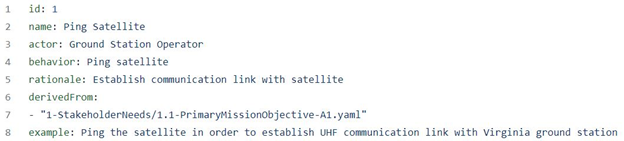
\includegraphics[width=13.75 cm]{assets/user_story.png}
    \caption{Example YAML file}
	\label{fig:example_yaml}
    \end{figure}   
\unskip

%%%%%%%%%%%%%%%%%%%%%%%%%%%%%%%%%%%%%%%%%%
\section{Architecture Implementation}
The implementation of M30ML serves as the basis for SeaLion mission architecture.  Presented here are the various elements, components, and products generated that is stored on the sealion-mission-architecture GitHub page \cite{sealion_mission_architecture}.  At the time of publication of this article, the implementation of the SeaLion mission architecture was done to the prior mission parameters where the SeaLion CubeSat was designed for a short lifespan compared to now greatly extended planned lifespan.  Since the mission parameters was changed rather recently prior to publication, the architecture had yet to be updated for them.

\subsection{File Structure}
The SeaLion mission architecture is organized into two main folders of architecture and of components \cite{sealion_mission_architecture}.  Architecture contains the references, stakeholder needs, user stories, and data structures shown in figure \ref{fig:reference_file}.  Components, as the name implies, contains the components and subcomponents of the CubeSat.  For the focus of this article, the architecture folder is the primary concern.  Components is currently a work in progress at time of publication of this article and will be addressed with future required work.  For the mission architecture shown in figure \ref{fig:folders}, generally data structures are derived from user stories.  Further, user stories are subsequently derived from stakeholder needs with their respective references.

\begin{figure}[H]
    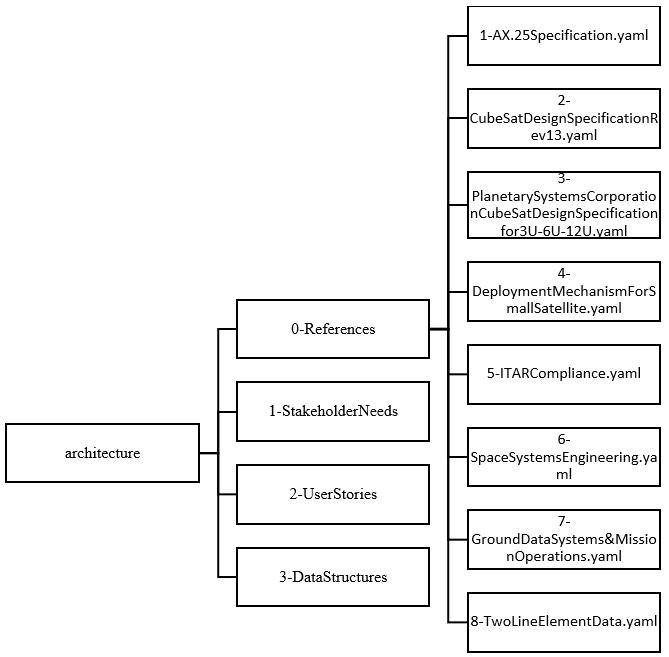
\includegraphics[width=10.5 cm]{assets/reference_file.png}
    \caption{References file structure}
	\label{fig:reference_file}
    \end{figure}   
\unskip

References are simply stored reference material such as standards, specifications books, etc.  They are very simple two-line YAML files as shown in figure \ref{fig:reference_yaml}.  This creates a continued link between the YAML files within their respective folders from which documents can be updated seamlessly.  Information changed within one file can interact with other files.  All YAML references files in the mission architecture at the time of article's publication is listed within figure \ref{fig:reference_file}. 

\begin{figure}[H]
    
\includegraphics[width=13.75 cm]{assets/reference.png}
    \caption{References YAML file}
	\label{fig:reference_yaml}
    \end{figure}   
\unskip

\subsection{Stakeholder Needs}
The development of SeaLion's mission architecture is guided by a series of stakeholder needs \cite{sealion_dof}.  After SeaLion's project methodology documentation is committed to using M30ML based on YAML modelling tools, the first step is to identify all stakeholder needs.  The two primary stakeholders of SeaLion are ODU and the USCGA.  Their respective needs are classified from primary, secondary, and tertiary based on mission importance.

Stakeholder YAML files are stored in the '1-StakeholderNeeds' folder shown in figure \ref{fig:folders}.  Each file is numbered with a X.X number format with the first number designating if it's primary, secondary, or tertiary and the second number denoting a place within a list of that class (e.g., 1.1 would indicate primary stakeholder need 1).  In addition, the letter associated (e.g., A1, B1, C1, etc.) in the filename would also signify if it's a primary, secondary, or tertiary stakeholder need.  Each YAML file contains an id number, name, statement, and derivedFrom field shown in figure \ref{fig:stakeholder_yaml}.  Note the reference YAML file that has filed in the derivedFrom field that serves as the basis for the stakeholder need.  While not all stakeholder needs have it filled, it is available to be used as needed.  Figure \ref{fig:stakeholder_file} showcases all the YAML files stored in the stakeholders file folder.

\begin{figure}[H]
    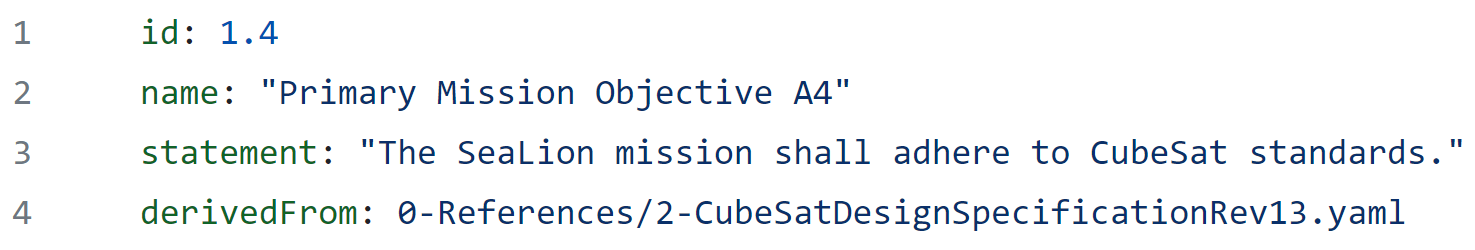
\includegraphics[width=13.75 cm]{assets/stakeholder.png}
    \caption{Stakeholder YAML file}
	\label{fig:stakeholder_yaml}
    \end{figure}   
\unskip

\begin{figure}[H]
    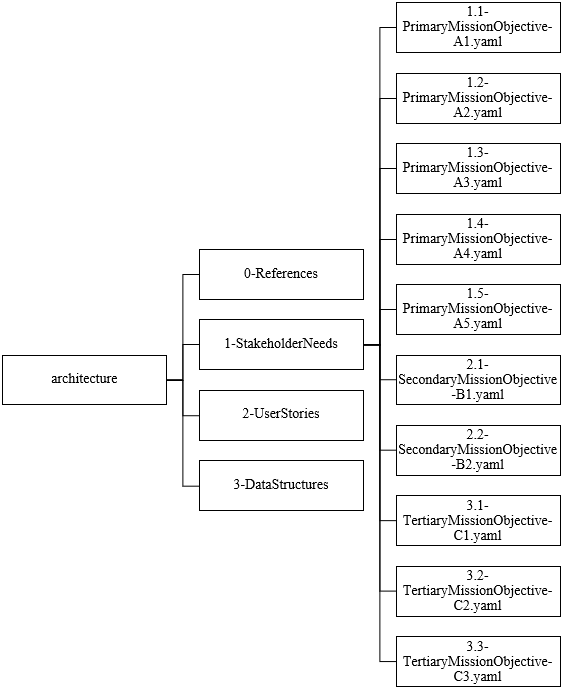
\includegraphics[width=10.5 cm]{assets/stakeholder_file.png}
    \caption{Stakeholders file structure}
	\label{fig:stakeholder_file}
    \end{figure}
	\noindent   
\unskip

Figure \ref{fig:uml_stakeholder} presents all the stakeholder needs via a unified modelling language (UML) diagram generated from the YAML files within the '1-StakeholderNeeds' folder.  The two primary stakeholders being ODU and the USCGA.  The generation of these diagrams via the YAML files presented herein showcases the docs-as-code approach.  YAML files structured as a code are then converted into human readable documents for presentation.

\begin{figure}[H]
    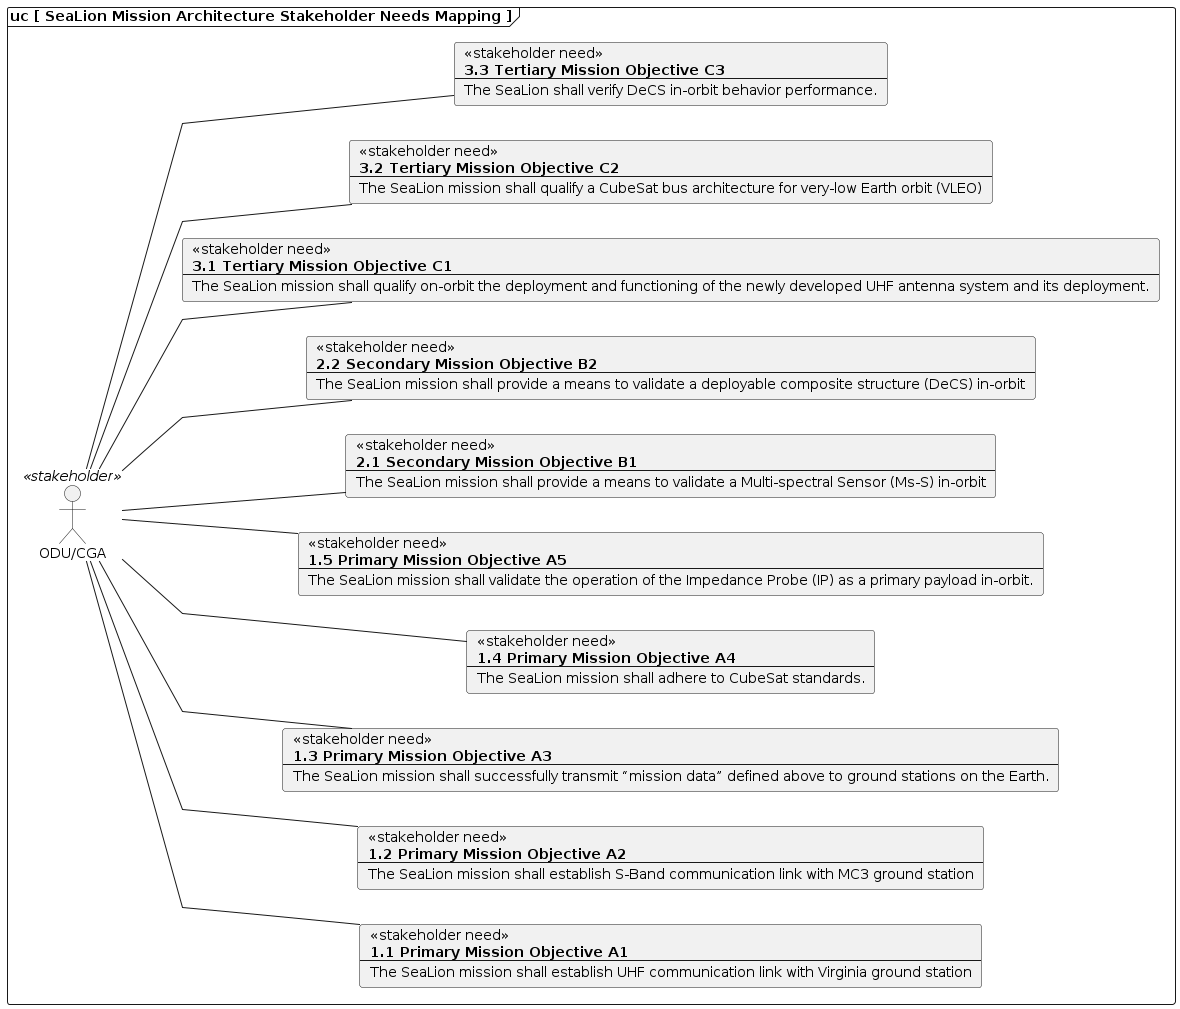
\includegraphics[width=13.75 cm]{assets/uml_stakeholder.png}
    \caption{Stakeholder UML Diagram}
	\label{fig:uml_stakeholder}
    \end{figure}   
\unskip

\subsection{User Stories}
Once the SeaLion mission architecture's stakeholder needs are identified and recorded, the stakeholder needs are then used to identify a series of user stories which then lead to design decisions captured in data structure and activity definitions \cite{sealion_page}.  These user stories are written from the perspective of the ground operator which would be a student from ODU who monitors and controls the functions of the SeaLion CubeSat.  User story YAML files are stored in the '2-UserStories' folder shown in figure \ref{fig:folders}.  These files are all given an ID number in no particular order of importance.  See the following figure \ref{fig:userstory_file} for the user story YAML file structure.

\begin{figure}[H]
    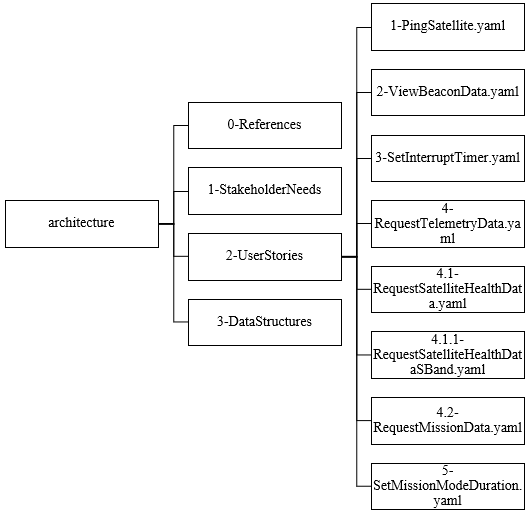
\includegraphics[width=10.5 cm]{assets/userstory_file.png}
    \caption{User stories file structure}
	\label{fig:userstory_file}
    \end{figure}
	\noindent   
\unskip

As an example, the second user story desire is to “verify that satellite is operating nominally” \cite{sealion_mission_architecture}.  Its full statement, derived from the actor, behavior, and rationale, would read “as a Ground Station Operator I want to view satellite beacon data (alternating between health and mission data), received via UHF so that I can verify that satellite is operating nominally” \cite{sealion_page}.  Its associated YAML file named '2-ViewBeaconData.yaml' is presented in figure \ref{fig:view_beacon}.  Note that this user story is derived from stakeholder needs A1, A3, A5, B1, B2, C1, C2, and C3 which are stakeholder needs mentioned in the prior section detailing stakeholder needs.  Additionally, the example statement is cut-off in figure \ref{fig:view_beacon} for readability.  It should read in full as “View satellite beacon data (health or mission data) to verify that state vector correspond with expected orbit profile and/or to validate that a mission mode was successful”.  This satellite beacon data, transmitted via UHF, is used to validate that any and all functions of the satellite are operating nominally or as planned in respect to their payloads hence the large derivedFrom list in the associated YAML file.

\begin{figure}[H]
    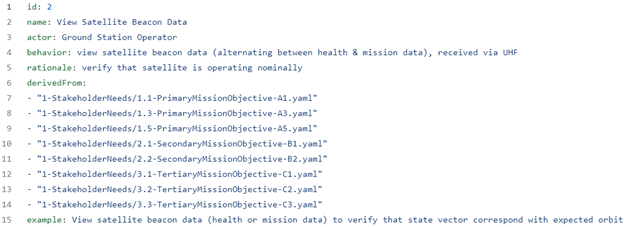
\includegraphics[width=13.75 cm]{assets/view_beacon.png}
    \caption{View Beacon YAML structure}
	\label{fig:view_beacon}
    \end{figure}
	\noindent   
\unskip

Figure \ref{fig:uml_userstory} and figure \ref{fig:uml_userstory2} are UML diagrams generated using the YAML files stored in the '2-UserStories' folder.  Figure \ref{fig:uml_userstory} is an excerpt of mapping of stakeholder needs to user stories.  Figure \ref{fig:uml_userstory2} is the user stories presented in a use case diagram to showcase what the ground station operator needs to perform.  The generation of these diagrams via the YAML files presented herein showcases the docs-as-code approach.  YAML files structured as a code are then converted into human readable documents for presentation.

\begin{figure}[H]
    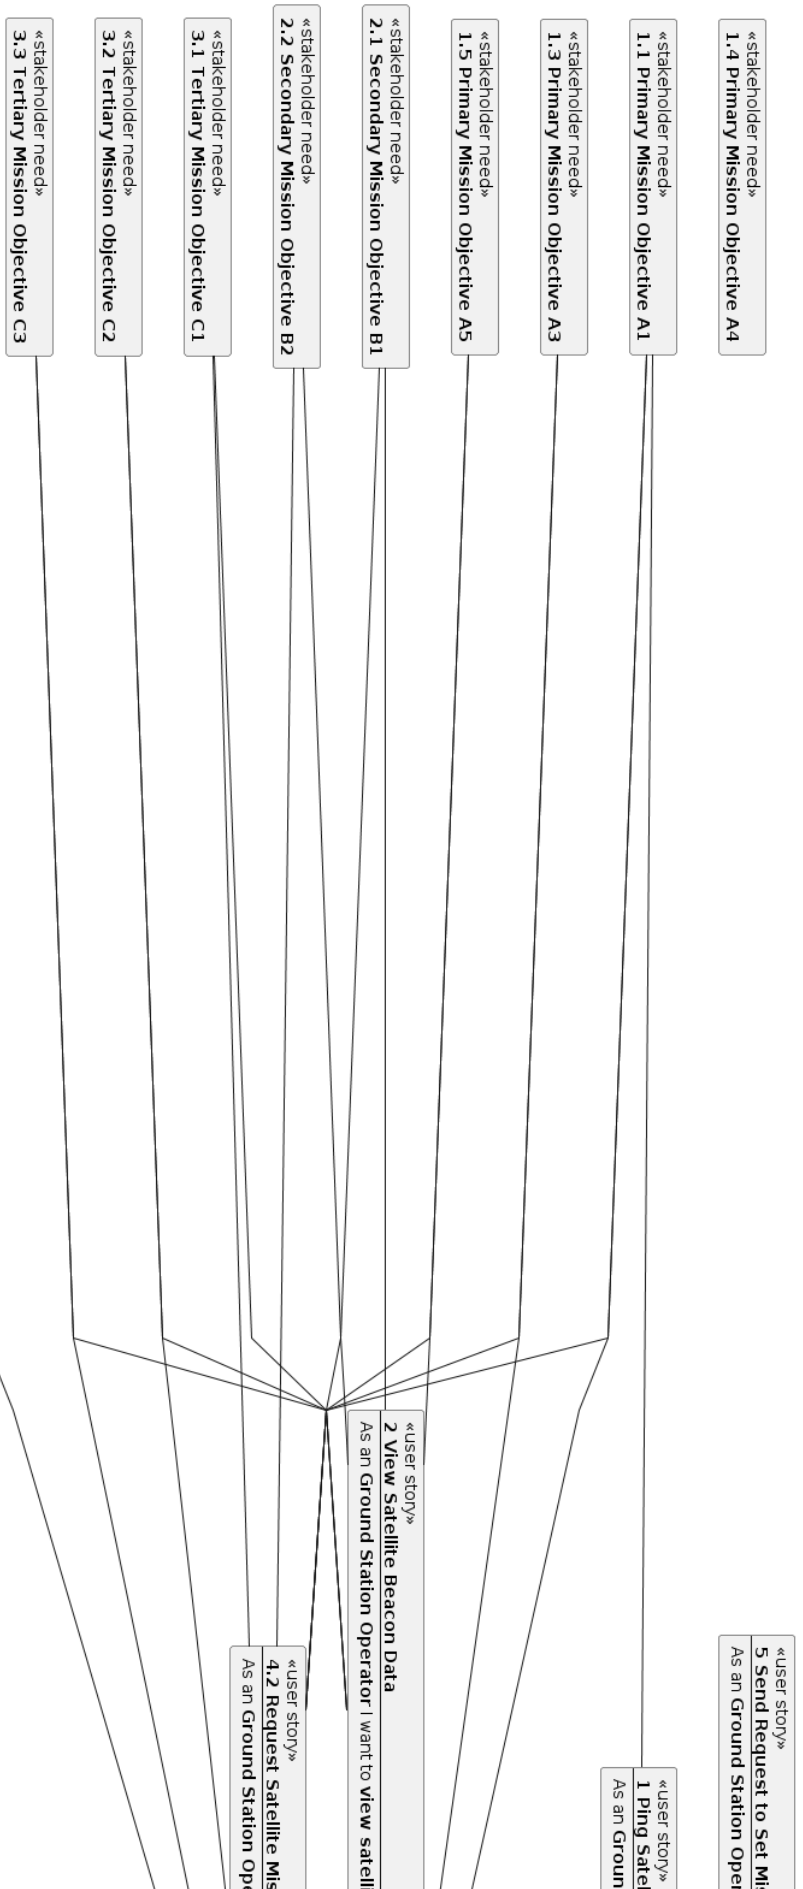
\includegraphics[height=21 cm]{assets/uml_userstory.png}
    \caption{Excerpt of UML diagram of user stories}
	\label{fig:uml_userstory}
    \end{figure}   
\unskip

\begin{figure}[H]
    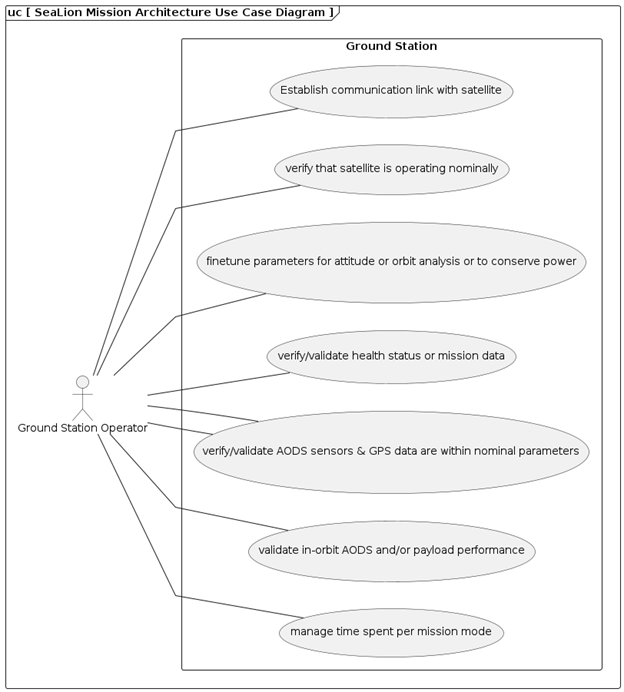
\includegraphics[width=13.75 cm]{assets/uml_userstory2.png}
    \caption{UML diagram of ground station operator}
	\label{fig:uml_userstory2}
    \end{figure}   
\unskip

\subsection{Data Structures}
User stories once identified will then lead to design decisions captured in data structures and activity definitions.  These data structures are the data that would be transmitted back and forth between ground station operator and CubeSat.  Data structure YAML files are stored in the '3-DataStructures' folder shown in figure \ref{fig:folders}.  Each data structure YAML has name, purpose, template, elements, and derived from elements as shown in figure \ref{fig:datastructure} as an example.  Name and purpose are for identification and stated use case.  Template lists out all the elements that are called out via their identifying key.  Elements detail the specific values as part of the data structure; each element has their own identifying information and descriptions.  The derived from field is used to tie back the data structure to a user story YAML file should it be applicable.  Table \ref{tab:datastructure} is a table generated from the YAML file shown in figure \ref{fig:datastructure} for documentation purposes.  Figure \ref{fig:datastructure_file} details the file structure under the 3-DataStructures' folder.

\begin{table}[H] 
	\caption{Data Structure of Packet}
	\label{tab:datastructure}
	\newcolumntype{C}{>{\centering\arraybackslash}X}
	\begin{tabularx}{\textwidth}{CCCC}
	\toprule
	\textbf{Field}  & \textbf{Type}  & \textbf{Description}\\
	\midrule
	call\_sign           & string         & Identifying call sign for the Sealion mission.                                                                         \\ \hline
	battery\_health      & float          & Percent value indicating the remaining charge of the batteries.                                                        \\ \hline
	temperature\_battery & float          & The temperature of the battery. Units in Kelvin.                                                                       \\ \hline
	mode                 & integer        & Integer value indicating current mission mode. 0 = Safe, 1 = mission mode 1, 2 =   mission mode 2, 3 = mission mode 3. \\ \hline
	state\_vector        & ECIStateVector & ECI state vector from orbit propogator at time of beacon. \\    
	\bottomrule
	\end{tabularx}
\end{table}

\begin{figure}[H]
    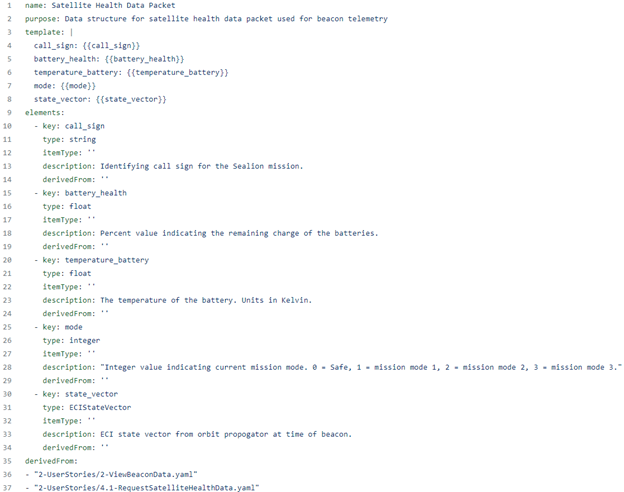
\includegraphics[width=13.75 cm]{assets/datastructure.png}
    \caption{Satellite Health Data Structure}
	\label{fig:datastructure}
    \end{figure}   
\unskip

\begin{figure}[H]
    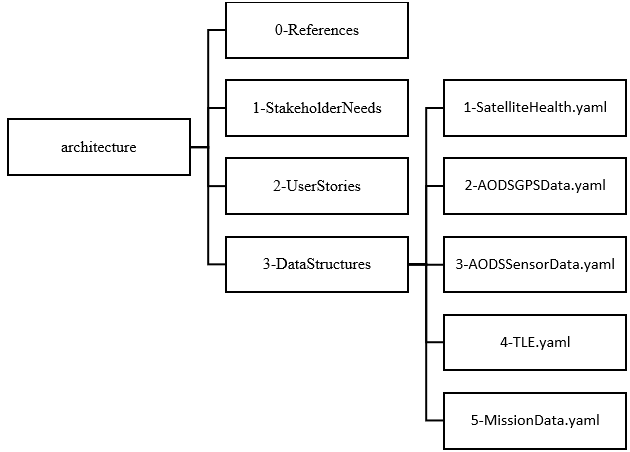
\includegraphics[width=10.5 cm]{assets/datastructure_file.png}
    \caption{Data structure File Structure}
	\label{fig:datastructure_file}
    \end{figure}
	\noindent   
\unskip

As shown in figure \ref{fig:datastructure}, the data structure, with YAML file named '1-SatelliteHealth.yaml' is for determining the satellite's health.  This data would be transmitted with the beacon data to be received by the ground station operator.  Note that this data structure is derived from the user stories 2 and 4.1 described in the prior section detailing user stories.  These user stories detail the ground station operator's tasks to view the satellite beacon data and to request the satellite health data packet so that the operator can verify that AODS sensors and GPS data are within nominal parameters.  Table \ref{tab:datastructure} details the various fields that would be required in this beacon data packet to accomplish the aforementioned tasks.

\begin{figure}[H]
    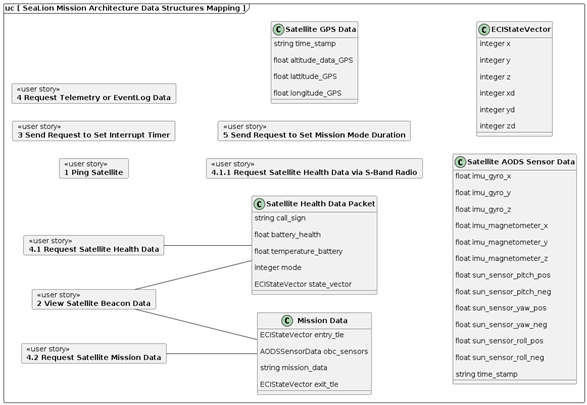
\includegraphics[width=13.75 cm]{assets/uml_datastructure.png}
    \caption{UML Diagram of Data Structures}
	\label{fig:uml_datastructure}
    \end{figure}   
\unskip

Figure \ref{fig:uml_datastructure} is a UML diagram of mapping of user stories to data structures generated from the YAML file shown in figure \ref{fig:datastructure}.  Note that not every data structure is linked to a user story.  These unlinked data structures are necessary to CubeSat functionality without being linked to the stakeholders and user story chain.  The generation of this diagram and the tables via the YAML files presented herein showcases the docs-as-code approach.  YAML files structured as a code are then converted into human readable documents for presentation.

\subsection{Document Generation}
As noted multiple times throughout this article, there have been a number of figures and tables generated from the YAML files placed within the SeaLion mission architecture GitHub repository.  Many of the figures are UML diagrams that are auto-generated artifacts rendered from the M30ML modeling language and formatted using the Liquid template language.  This is how the docs-as-code approach is implemented.  YAML code files are used to generate documents for information sharing between group members.  This means that any changes made to the SeaLion mission architecture model can immediately be used to generate new documents.  Whether it be diagrams, tables, or text, continuous updating is ensured that any changes affecting dependencies within the mission architecture are kept in sync.  YAML files are automatically processed using templates langauge (e.g., Jinja2) via a build shell script.  This also means that content of the model and formatting of documents are decoupled.  The model is formatting-agnostic for documentation purposes as this is handled by the template language.  A conference proceeding manuscript presented in AIAA SciTech 2023 was created purely by a docs-as-code format \cite{scitech_proceeding}.  The team used a LaTeX template to automatically format the manuscript to the conference guidelines and subsequently inject items such as the generated diagrams, tables, and references directly into the manuscript.

%%%%%%%%%%%%%%%%%%%%%%%%%%%%%%%%%%%%%%%%%%
\section{M30ML Extensions for Component Implementation}
The implementation of M30ML for components, at the time of this article's publication, is currently in-process of integrating content information into the model.  A brief description of current component implementation into the SeaLion model is provided.  However, the model content mentioned herein is subjected to change.

\subsection{Distributed OSHW Framework}
The current SeaLion mission architecture repository, at time of article publication, for components is “structured as a Distributed OSHW Framework (DOF) - component for defining the contents of the Mission concept of operations (ConOps) as a collection of nested subcomponents, component interfaces, and component functions for generating bill of materials (BOMs) and assembly instructions for the SeaLion CubeSat” \cite{sealion_mission_architecture}.  The DOF pillars are based on Open Source Hardware (OSHW) principals \cite{mach30_git}.  The implementation methodology presented herein is an extension of M30ML specifically for the use of modelling a CubeSat design.  
  
The SeaLion mission architecture repostiory has a components folder dedicated to its namesake.  Inside the components folder of the repository are two subfolders; one labeled with 'sealion-cubesat' and another labeled with 'sealion-ground-station'.  Each of those folders would contain a components folder and subsequently those individual labeled components can have their own components folder.  Thus, a chain of components and subcomponents can be created as illustrated in figure \ref{fig:components_file}.  A parts YAML file in each components folder details what the subcomponents would be.  An excerpt example for the main SeaLion cubesat is provided in figure \ref{fig:components} that is associated with the file folders shown in figure \ref{fig:components_file}.

\begin{figure}[H]
    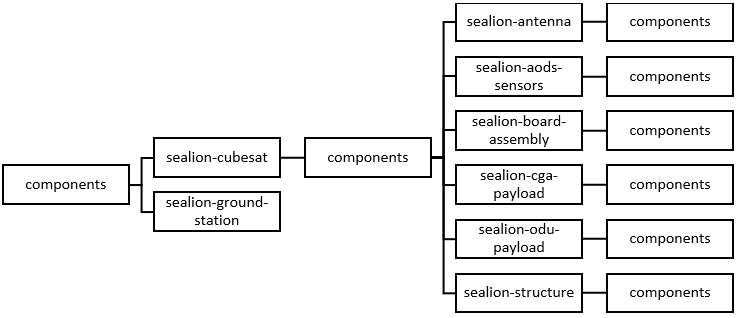
\includegraphics[width=10.5 cm]{assets/components_file.png}
    \caption{Components Folder File Structure}
	\label{fig:components_file}
    \end{figure}   
\unskip

\begin{figure}[H]
    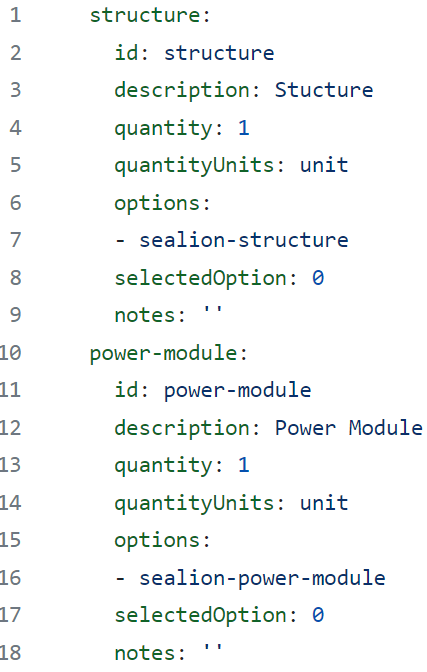
\includegraphics[width=5 cm]{assets/components.png}
    \caption{Component YAML File}
	\label{fig:components}
    \end{figure}   
\unskip

\subsection{Component Data Structure and File Implementation}
A series of YAML files for components have been created.  Figure \ref{fig:components} showcases the parts YAML file, however, parts is only one element of the component's data structure thus far.  Showcased in table \ref{tab:component_data} is the entire component data structure from the SeaLion DOF templates \cite{sealion_dof}.  There are a number of component data structures prepared, however, it is still in contention whether or not all of these data structures will be used.  The SeaLion DOF templates document have been generated in the DOF repository \cite{sealion_dof}.  The data structures created are as follows:

\begin{itemize}
	\item	Component: Represents the smallest logical element in an OSHW project. A Component may be a project in its own right (with a sub-component hierarchy) or may be nested as a sub-component in the "source" of another component.
	\item	Component List Item: Identifies a part or tool used in the fabrication of the component. Parts and tools are defined by their source material in the components list.
	\item	Activity Step: Defines a single step in an activity (e.g., assembly instructions).
	\item	Parameter: Defines a data structure for an input or output of a component function.
	\item	Function: Defines a data structure for a component function.
	\item	Interface List Item: Identifies an interface on a part or tool.
\end{itemize}

\begin{table}[H] 
	\caption{Component Data Structure}
	\label{tab:component_data}
	\newcolumntype{C}{>{\centering\arraybackslash}X}
	\begin{adjustwidth}{-\extralength}{0cm}
	\newcolumntype{C}{>{\centering\arraybackslash}X}
	\begin{tabularx}{\fulllength}{CCCC}
	\toprule
	\textbf{Field}  & \textbf{Type}  & \textbf{Item Type}  & \textbf{Description}\\
	\midrule
	name          & string     &                       & Source   representation of the component's name. Format = single word, only lowercase   letters, and may contain hyphens and underscores.                                   \\ \hline
	version       & string     &                       & Version   number of the component's source. Format = x.x.x per semantic versioning   guidelines.                                                                            \\ \hline
	description   & string     &                       & Human   readable representation of the component's name. Typically used in rendered   documentation referencing the component.                                              \\ \hline
	license       & string     &                       & List of   licenses used within the component's source. Format = SPDX license   expression.                                                                                  \\ \hline
	author        & string     &                       & Identifies   author (e.g. owner of source intellectual property). Format (email and   website are optional)= Author Name \textless{}email address\textgreater (website URL) \\ \hline
	dependencies  & dictionary & string                & Per   NPM/Yarn. Key = dependency name. Value = Semantic versioning version string.                                                                                          \\ \hline
	components    & dictionary & Component             & Listing   of sub-components directly owned by this component. Key = sub-component's   name. Value = sub-component's data structure.                                         \\ \hline
	parts         & dictionary & Component   List Item & Listing   of the component's parts (and substitutions) defined as sub-components. Key =   part's id. Value = part's key data.                                               \\ \hline
	functions     & list       & Function              & Listing   of component functions.                                                                                                                                           \\ \hline
	tools         & dictionary & Component   List Item & Listing   of the required tools (and substitutions) defined as sub-components. Key =   tool's id. Value = tool's key data.                                                  \\ \hline
	precautions   & list       & string                & Listing   of caution statements (e.g. safety warnings) for the component.                                                                                                   \\ \hline
	assemblySteps & list       & Activity   Step       & Sequence   of steps required to assemble the component. \\
	\bottomrule
	\end{tabularx}
	\end{adjustwidth}
\end{table}

The initial goal is to list the components of the SeaLion CubeSat and to generate assembly steps for them.  Through which the architecture can provide detailed documentation to assemble the SeaLion CubeSat.  These assembly instructions would also be generated through the SeaLion mission architecture repository much akin to other documents for SeaLion.  Thus, it creates a human readable document from the YAML files code as per the docs-as-code approach.

Eventually, the purpose of all these component data structures is to also create a N2 diagram.  A N2 diagram is used to “capture the interfaces, mechanical and electrical, for all components of the satellite obtained through the mapping process” \cite{asundi13_cubes}.  An example has been provided in figure \ref{fig:N2}.  The end goal is that the architecture would use interfaces and junctions within the YAML files code to automatically generate an N2 diagram.  Thus, it allows for continuous updating that ensures that any changes affecting dependencies within the mission architecture are kept in sync.  This would allow for a team to identify “areas where conflicts could arise in interfaces, and highlights input and output dependency assumptions and requirements” \cite{asundi13_cubes}.  Thus, leading to higher efficacy in planning the development and assembly of the satellite.

\begin{figure}[H]
    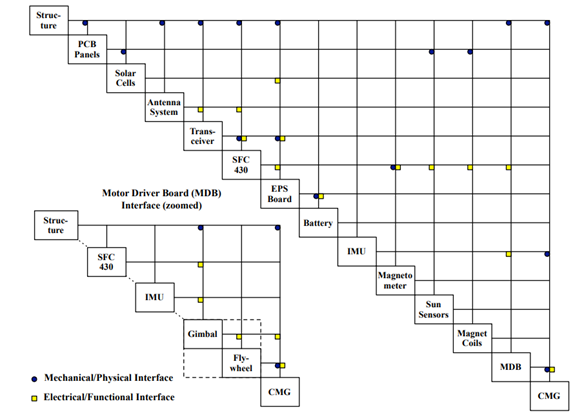
\includegraphics[width=13.75 cm]{assets/N2.png}
    \caption{N2 Chart Example}
	\label{fig:N2}
    \end{figure}   
\unskip

\section{Future Work and Observations}
Implementation of the overall mission architecture has been successful for the original mission profile.  Future work includes adapting the mission architecture to the new mission profile from the launch delay.  For example, it has spawned a tradestudy for rechargable batteries and solar panals.  However, the original mission architecture does not require extensive rework since many attributes are similar.  The mission architecture requires only a few sessions between team members to make adaptations.  All documentation would be automatically updated to reflect these changes per the docs-as-code approach which will eliminate additional work in that category.

Extensions to the DOF data model are also under development for enabling additional use cases, such as the N2 chart, for cubesat systems engineering \cite{sealion_dof}.  This extended data model would serve as a self-describing specification that new cubesat projects could adopt for their own cubesat missions, whereby the SeaLion mission would serve as the first reference implementation.  Additionally, training material will be developed around this new data model in efforts to help guide incoming CubeSat developers.  Multiple team members of the SeaLion mission have been able to quickly learn the methodology of using the docs-as-code approach within a short training session with an experienced member.  However, a fully realized tutorial would be beneficial to allow for self-learning.  Current guides are lists of definitions and format guides rather than a step by step tutorial on using the approach which has caused confusion amongst members that attempted to self-learn.

Additionally, observations from the implmentation of the docs-as-code approach noted that an effective communication plan between team members is key to the overall effectiveness of the mission architecture.  Team members focused on specific parts of the CubeSat's development (e.g., structure, payload, etc.) are required to add all necessary content to the architecture.  If team members are unavailable due to other more important obligations (e.g., universtiy courses), it can cause considerable delays in the architecture's completion.  The SeaLion mission architecture team necessitated frequent meetings with individual team members to gather the necessary content for the architecture to capture all legacy work.  Legacy work being design decisions made prior to the architecture model's introduction.  In an ideal case, a mission architecture would be formatted prior to any major design decision so that all team members can work directly to the architecture model rather than adapting legacy work to the model.

%%%%%%%%%%%%%%%%%%%%%%%%%%%%%%%%%%%%%%%%%%
\section{Conclusion}
The SeaLion mission architecture team used MBSE with a docs-as-code approach to the SeaLion project. This was done in efforts to reduce the friction and disconnect associated with traditional systems engineering for CubeSat developers.  This is particularly important when CubeSat projects are growing more numerous with many of their respective team members being new to space systems development.  The methodology presented herein has accomplished the ability to create individual elements of the architecture in an human readable code that is also easy to make revisions to and persists on a local file system.  Even for those who are unfamiliar with coding software or methodology.  Thus, minimal training is required for usage.  The mission architecture presented captures the necessary information required of its original mission profile while also generating documents for easy presentation as well.  Further work is required to create tutorials to train new users in a self-learning environment.  Other future work includes the components implementation to faciliate interfaces and junctions for proper component relationships and planning, DOF data model extensions, and adaption to the new mission profile.  Additionally, new users to this methodology should establish an effective team communication plan at the beginning of a project in order to prevent delays or rework in the creation of a mission architecture.    

%%%%%%%%%%%%%%%%%%%%%%%%%%%%%%%%%%%%%%%%%%
\vspace{6pt} 

%%%%%%%%%%%%%%%%%%%%%%%%%%%%%%%%%%%%%%%%%%
%\authorcontributions{For research articles with several authors, a short paragraph specifying their individual contributions must be provided. The following statements should be used ``Conceptualization, X.X. and Y.Y.; methodology, X.X.; software, X.X.; validation, X.X., Y.Y. and Z.Z.; formal analysis, X.X.; investigation, X.X.; resources, X.X.; data curation, X.X.; writing---original draft preparation, X.X.; writing---review and editing, X.X.; visualization, X.X.; supervision, X.X.; project administration, X.X.; funding acquisition, Y.Y. All authors have read and agreed to the published version of the manuscript.'', please turn to the  \href{http://img.mdpi.org/data/contributor-role-instruction.pdf}{CRediT taxonomy} for the term explanation. Authorship must be limited to those who have contributed substantially to the work~reported.}

\funding{This research received no external funding.}

%\dataavailability{We encourage all authors of articles published in MDPI journals to share their research data. In this section, please provide details regarding where data supporting reported results can be found, including links to publicly archived datasets analyzed or generated during the study. Where no new data were created, or where data is unavailable due to privacy or ethical re-strictions, a statement is still required. Suggested Data Availability Statements are available in section “MDPI Research Data Policies” at \url{https://www.mdpi.com/ethics}.} 

\acknowledgments{Special thanks to the SeaLion Project Team}

\conflictsofinterest{The authors declare no conflict of interest.} 

%%%%%%%%%%%%%%%%%%%%%%%%%%%%%%%%%%%%%%%%%%
%% Only for journal Encyclopedia
%\entrylink{The Link to this entry published on the encyclopedia platform.}

\abbreviations{Abbreviations}{
The following abbreviations are used in this manuscript:\\

\noindent 
\begin{tabular}{@{}ll}
1U &	1-Unit\\
2U &	2-Unit\\
3U &	3-Unit\\
AC &	Alternating Current\\
AFIT &	 Air Force Institute of Technology \\
AIAA &	American Institute of Aeronautics and Astronautics \\
AODS &	Altitude and Orbit Determination System\\
BOM &	Bill of Material\\
ConOps &	Concept of Operations\\
COTS &	Commerical Off-the-Shelf\\
DeCS &	Deployable Composite Structure\\
DOA &	Dead on Arrival\\
doctools &	Dcoument Tools\\
DOF &	Distributed OSHW Framework \\
EVR &	Event\\
FPP &	F Prime Prime\\
GPS &	Global Positioning System\\
ISS &	International Space Station\\
M30ML &	Mach 30 Modelling Language\\
MBSE &	Model Based Systems Engineering\\
MC3 &	Mobile CubeSat Command and Control \\
Me-S &	Multi-spectral Sensor \\
NRL &	Naval Research Laboratory\\
ODU &	Old Dominion University\\
OML &	Ontological Modeling Language \\
OSHW &	Open Source Hardware\\
OWL2 &	Web Ontology Language 2 \\
Q4 &	Quarter Four\\
SPADE &	Space PlasmADiagnostic suitE\\
SWRL &	Semantic Web Rule Language \\
UHF &	Ultra High Frequency \\
UML & Unified Modelling Language\\
USCGA &	United States Coast Guard Academy\\
VLEO &	Very Low Earth Orbit\\
WFF &	Wallops Flight Facility\\
XMI & XML Metadata Interchange
\end{tabular}
}

%%%%%%%%%%%%%%%%%%%%%%%%%%%%%%%%%%%%%%%%%%
\begin{adjustwidth}{-\extralength}{0cm}
%\printendnotes[custom] % Un-comment to print a list of endnotes

\reftitle{References}

% Please provide either the correct journal abbreviation (e.g. according to the “List of Title Word Abbreviations” http://www.issn.org/services/online-services/access-to-the-ltwa/) or the full name of the journal.
% Citations and References in Supplementary files are permitted provided that they also appear in the reference list here. 

%=====================================
% References, variant A: external bibliography
%=====================================
%\bibliography{mdpi-manuscript-references}

%=====================================
% References, variant B: internal bibliography
%=====================================
\begin{thebibliography}{999}
    \bibitem{architecting_spacecraft}Friedenthal, S. \& Oster, C. Architecting spacecraft with SysML.  (2017)
    \bibitem{nasa_handbook}NASA NASA System Engineering Handbook. (NASA,2016)
    \bibitem{asundi13_cubes}Asundi, S. \& Fitz-Coy, N. CubeSat mission design based on a systems engineering approach. {\em 2013 IEEE Aerospace Conference}. pp. nil (2013,3), http://dx.doi.org/10.1109/AERO.2013.6496900
    \bibitem{scitech_proceeding}Sean Marquez, S. Model-Based CubeSat Flight-Software Architecture using a Docs-as-Code approach. {\em AIAA Scitech Conference 2023}. (2023,1), https://arc.aiaa.org/doi/10.2514/6.2023-1126
    \bibitem{cds_rev14}The CubeSat Program, C. CubeSat Design Specification Rev. 14. (The CubeSat Program, Cal Poly SLO,2022)
    \bibitem{sealion_cdr}Academy, O. Critical Design Review: Mission SeaLion - ODU/CGA 3U CubeSat.  (2022)
    \bibitem{heidt_new}Heidt, H., Puig-Suari, J., Moore, A., Nakasuka, S. \& Twiggs, R. CubeSat - A new generation of picosatellite for education and industry low-cost space experimentation. {\em AIAA/USU Annual Conference On Small Satellites, 12th, Utah State University, Logan; UNITED STATES; 21-24 Aug.2000}. (2000,8), https://www.proquest.com/conference-papers-proceedings/cubesat-new-generation-picosatellite-education/docview/27219077/se-2
    \bibitem{sealion_cdr}Academy, O. Critical Design Review: Mission SeaLion - ODU/CGA 3U CubeSat.  (2022)
    \bibitem{heidt_new}Heidt, H., Puig-Suari, J., Moore, A., Nakasuka, S. \& Twiggs, R. CubeSat - A new generation of picosatellite for education and industry low-cost space experimentation. {\em AIAA/USU Annual Conference On Small Satellites, 12th, Utah State University, Logan; UNITED STATES; 21-24 Aug.2000}. (2000,8), https://www.proquest.com/conference-papers-proceedings/cubesat-new-generation-picosatellite-education/docview/27219077/se-2
    \bibitem{swartwout_data}Swartwout, M. CubeSat Database.  (2021), https://sites.google.com/a/slu.edu/swartwout/cubesat-database
    \bibitem{pumpkin_cubesat}Shop, C. Pumpkin CubeSat Kits.  (2023,3), https://www.cubesatshop.com/product/pumpkin-cubesat-kits/
    \bibitem{cubesat_handbook}Cappelletti Cubesat handbook: From mission design to operations. (Elsevier Science \& Technology,2020)
    \bibitem{reliving_24}Swartwout, M. Reliving 24 Years in the Next 12 Minutes: A Statistical and Personal History of University-Class Satellites.  (2018), https://digitalcommons.usu.edu/cgi/viewcontent.cgi?article=4277\&context=smallsat
    \bibitem{aalto}Praks AALTO-1 earth observation cubesat mission — Educational outcomes. {\em IEEE International Geoscience And Remote Sensing Symposium (IGARSS)}. (2015)
    \bibitem{howtosetup}Berthoud, M. How to Set Up a CubeSat Project - Preliminary Survey Results. {\em 30th Annual AIAA/USU Conference On Small Satellites}. (2016)
    \bibitem{sealion_mission_architecture}Team, S. SeaLion Mission Architecture. (Old Dominion University,2022), https://github.com/ODU-CGA-CubeSat/sealion-mission-architecture
    \bibitem{caesar_model_based_approach}David Wagner CAESAR Model-Based Approach to Harness Design. {\em Proceedings Of IEEE Aerospace Conference}. (2020,3)
    \bibitem{ibm_mbse}Brown, B. Model-based systems engineering: Revolution or evolution?.  (2011,12)
    \bibitem{docs_as_code}Holscher, E. Docs as Code.  (2022), https://www.writethedocs.org/guide/docs-as-code/
    \bibitem{mach30_git}Simmons, J. Mach30 Modeling Language. (Mach30 Foundation,2022), https://github.com/Mach30/m30ml
    \bibitem{sys_ml}Partners, S. SysML Specifications.  (2023), https://sysml.org/sysml-specs/
    \bibitem{sys_ml2}Submission Team, S. SysML-v2-Release.  (2023), https://github.com/Systems-Modeling/SysML-v2-Release
    \bibitem{plantuml}PlantUML PlantUML.  (2023), https://plantuml.com/
    \bibitem{oml_language}Maged Elaasar, N. Ontological Modeling Language: Origin and Rationale.  (2022), http://www.opencaesar.io/oml/
    \bibitem{oml_origin_and_rationale}Jenkinis, S. Ontological Modeling Language 1.4.  (2022), http://www.opencaesar.io/imce/2021/06/19/OML-Origin-and-Rationale.html
    \bibitem{sealion_dof}Team, S. Distributed OSHW Framework (DOF). (Old Dominion University,2023), https://odu-cga-cubesat.github.io/dof-cubesat/
    \bibitem{sealion_page}Team, S. SeaLion Mission Architecture. (Old Dominion University,2023), https://odu-cga-cubesat.github.io/sealion-mission-architecture/
    \bibitem{linkml}Mungall, C. LinkML model your data. {\em LinkML}., https://linkml.io/
    \bibitem{younse_cameron_bradley_2021}Younse, P., Cameron, J. \& Bradley, T. Comparative analysis of model-based and traditional systems engineering approaches for architecting a robotic space system through Automatic Information Transfer. {\em IEEE Access}. \textbf{9} pp. 107476-107492 (2021)
    \bibitem{call_herber_2022}Call, D. \& Herber, D. Applicability of the diffusion of innovation theory to accelerate model-based systems engineering adoption. {\em Systems Engineering}. \textbf{25}, 574-583 (2022)
    \bibitem{mazzini}Mazzini, S., Tronci, E., Paccagnini, C. \& Olive, X. A Model-Based methodology to support the Space System Engineering (MBSSE). {\em ERTS2 2010, Embedded Real Time Software \& Systems}. (2010,5), https://hal.science/hal-02267836
    \bibitem{esa}ESA Model-based system engineering. , https://www.esa.int/Enabling\_Support/Preparing\_for\_the\_Future/Discovery\_and\_Preparation/Model-based\_system\_engineering
    \bibitem{nottage_corns_2012}Nottage, D. \& Corns, S. Application of model-based systems engineering on a university satellite design team. {\em Procedia Computer Science}. \textbf{8} pp. 207-213 (2012)
    \bibitem{kaslow}Kaslow, D., Ayres, B., Cahill, P., Hart, L. \& Yntema, R. Developing a CubeSat Model-Based System Engineering (MBSE) reference model — Interim status \#3. {\em 2017 IEEE Aerospace Conference}. pp. 1-15 (2017)
    \bibitem{structurizr}Structurizr Software architecture models as code. {\em Structurizr}., https://structurizr.org/
    \bibitem{f_prime_prime}Bocchino, R., Levison, J. \& Starch, M. FPP: A Modeling Language for F Prime. {\em 2022 IEEE Aerospace Conference (AERO)}. pp. 1-15 (2022)
    \bibitem{f_prime}NASA F' a flight software and embedded systems framework. {\em F'}., https://nasa.github.io/fprime/
\end{thebibliography}

% If authors have biography, please use the format below
%\section*{Short Biography of Authors}
%\bio
%{\raisebox{-0.35cm}{\includegraphics[width=3.5cm,height=5.3cm,clip,keepaspectratio]{Definitions/author1.pdf}}}
%{\textbf{Firstname Lastname} Biography of first author}
%
%\bio
%{\raisebox{-0.35cm}{\includegraphics[width=3.5cm,height=5.3cm,clip,keepaspectratio]{Definitions/author2.jpg}}}
%{\textbf{Firstname Lastname} Biography of second author}

% For the MDPI journals use author-date citation, please follow the formatting guidelines on http://www.mdpi.com/authors/references
% To cite two works by the same author: \citeauthor{ref-journal-1a} (\citeyear{ref-journal-1a}, \citeyear{ref-journal-1b}). This produces: Whittaker (1967, 1975)
% To cite two works by the same author with specific pages: \citeauthor{ref-journal-3a} (\citeyear{ref-journal-3a}, p. 328; \citeyear{ref-journal-3b}, p.475). This produces: Wong (1999, p. 328; 2000, p. 475)

%%%%%%%%%%%%%%%%%%%%%%%%%%%%%%%%%%%%%%%%%%
%% for journal Sci
%\reviewreports{\\
%Reviewer 1 comments and authors’ response\\
%Reviewer 2 comments and authors’ response\\
%Reviewer 3 comments and authors’ response
%}
%%%%%%%%%%%%%%%%%%%%%%%%%%%%%%%%%%%%%%%%%%
\PublishersNote{}
\end{adjustwidth}
\end{document}

